\section{附录}
\label{app:models}

\textbf{模型与动作接口。} 表~\ref{tab:models} 总结本文讨论的三个结构化决策
模型。只有 Laya 与 Vela 在本地运行；Jev 定义商业参考点，本文不评测。

\begin{table}[t]
\centering
\small
\caption{本文讨论的三个结构化决策模型。只有 Laya 与 Vela 在本地运行；
Jev 定义商业参考点，本文不评测。}
\label{tab:models}
\begin{tabular}{@{}p{1.3cm}p{3.7cm}p{4.4cm}p{3.7cm}@{}}
\toprule
模型 & 接口 & 训练路线 & 本文角色 \\
\midrule
Jev & 一次调用返回带类型的 \textsc{Noul}、\textsc{Choice} 与 \textsc{Score} 决策及概率 & TypeSafe 称其为 RLCD 与适当评分目标；完整配方未公开 & RLCD / System One 家族的参考点；未运行 \\
Laya 0.4.16 & ModernBERT-large 编码器加决策头，约 4.21 亿参数；\textsc{Noul}、\textsc{Choice}、\textsc{Score} & 上游称配方为 RLCD，使用 log、spherical 与 ranked probability 分数 & 所有实验中使用的开放 RLCD 模型 \\
Vela 2.0 0.3B & 22 层 ModernBERT，768 隐藏维，8{,}192 token；\textsc{Noul}、\textsc{Choice}、\textsc{Score}、\textsc{Span}、\textsc{Set} & 从 Decision-1.0-Kai 的 Choice 路径初始化，任务特定损失与路由数据；未称 RLCD & 接口匹配、配方不同的对照模型 \\
\bottomrule
\end{tabular}
\end{table}


\label{app:native}

\textbf{原生单动作基线。} 表~\ref{tab:native} 报告两个原生动作在
\texttt{search\_dev} 池上的准确率与平均每次调用延迟。这些数字定义了每个
搜索策略所比较的固定策略。两种表示的每次调用成本相近，因此适应度函数使用
调用次数，而不是模型特定的延迟项。峰值常驻内存用于记录 CPU-only 执行包络。

\begin{table}[t]
\centering
\small
\caption{60 行选择池（\texttt{search\_dev}，种子 17）上的原生单动作基线。
延迟是本地 CPU 上每次调用的均值，仅用于说明两种表示成本大致相同；它不用于
适应度函数。}
\label{tab:native}
\begin{tabular}{@{}llrrrrrr@{}}
\toprule
任务 & 模型 & $n$ & \textsc{Noul} 准确率 & \textsc{Choice} 准确率 & \textsc{Noul} ms & \textsc{Choice} ms & 峰值 RSS (MB) \\
\midrule
CodeXGLUE & Laya & 60 & 0.450 & 0.650 & 2304 & 2239 & 2114 \\
CodeXGLUE & Vela & 60 & 0.633 & 0.667 & 2437 & 2341 & 1931 \\
FinDVer & Laya & 59 & 0.712 & 0.644 & 2768 & 2741 & 2117 \\
FinDVer & Vela & 59 & 0.458 & 0.458 & 2394 & 2263 & 1795 \\
ProcessBench & Laya & 60 & 0.100 & -- & 2616 & -- & 2124 \\
ProcessBench & Vela & 60 & 0.100 & -- & 1577 & -- & 1747 \\
\bottomrule
\end{tabular}
\end{table}


\label{app:extra}

\textbf{互补性总览。} 图~\ref{fig:headroom} 可视化表~\ref{tab:complementarity}
背后的总修复与净修复计数，包括把 train 选出的方向原样应用到 dev 与 confirm。

\begin{figure}[t]
\centering
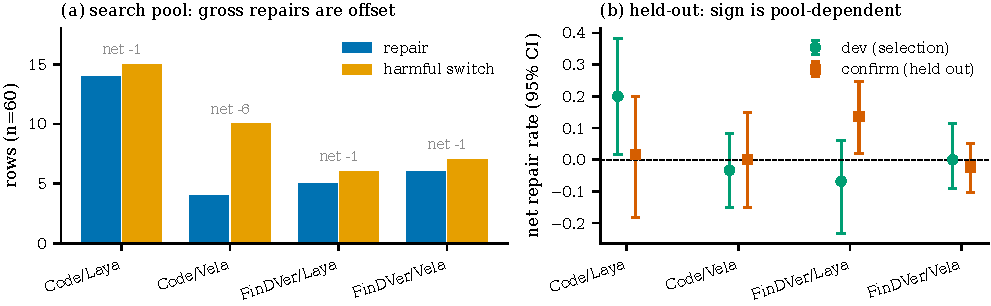
\includegraphics[width=0.96\linewidth]{../acl/figures/fig_headroom.pdf}
\caption{动作互补性。(a) 在训练池上，第二个动作修复错误，但也破坏正确答案；
每对柱上方印有净计数。(b) 同一 train 选出方向应用到 dev 与 confirm：净修复
的符号跨池变化，只有一个 confirm 单元的区间高于零。}
\label{fig:headroom}
\end{figure}

\textbf{修复轮廓。} 图~\ref{fig:repair} 显示第二个动作的修复率随 \noul{}
概率分箱的变化，分别给出训练、dev 与 confirm 池。每个点是该箱中 \noul{}
错误而 \choice{} 正确的行比例。当箱中至少有八行时印出箱计数。该图支持
第~\ref{sec:results} 节的论断：修复集中在概率中高段，而不是低置信度尾部。

\begin{figure}[t]
\centering
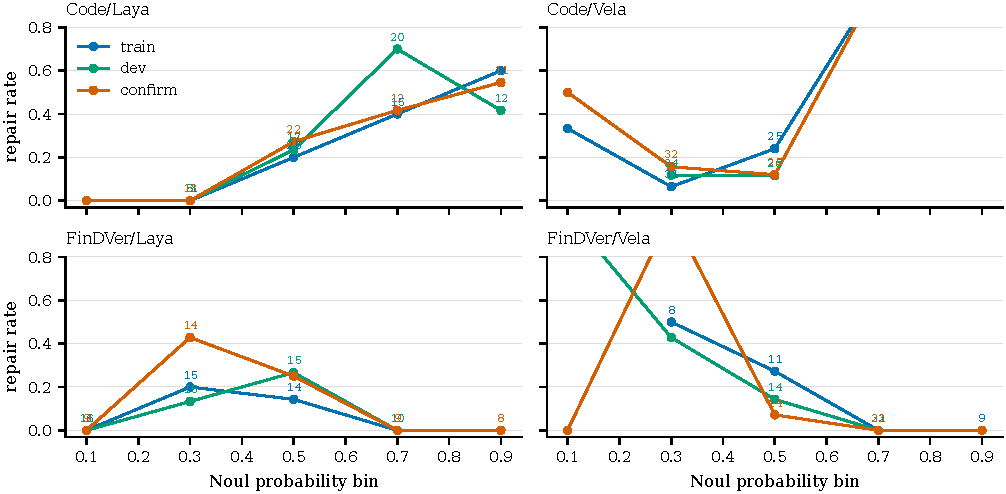
\includegraphics[width=0.96\linewidth]{../acl/figures/fig_repair_profile.pdf}
\caption{四个二元单元的修复率随 \noul{} 概率分箱的变化。最低箱中修复很少，
修复集中在 $p\in[0.4,0.8]$ 附近，而这正是置信度级联最不可能切换的地方。}
\label{fig:repair}
\end{figure}

\textbf{校准细节。} 表~\ref{tab:calibration} 报告校准及其与路由的关系；
图~\ref{fig:calibration} 画出四个二元单元在 confirm 上的可靠性图，包含温度
缩放前后。缩放参数在 \texttt{search\_train} 上拟合，原样应用到 confirm。
由于温度缩放是单调的，它改变数值概率，但不改变行的排序，因此也不改变路由
器可用的带策略集合。

\begin{table}[t]
\centering
\scriptsize
\setlength{\tabcolsep}{2.5pt}
\caption{\texttt{confirm} 上的校准及其与路由的关系。温度 $T$ 在
\texttt{search\_train} 上拟合；ECE 使用 15 个等宽箱。金标签 AUROC 是概率
排序当前动作正确性的能力；修复 AUROC 是它排序第二个动作可修复行的能力。
最后两列是在 \texttt{search\_dev} 上选择的带策略，分别用原始概率与温度
缩放概率得到的净修复。}
\label{tab:calibration}
\resizebox{\linewidth}{!}{%
\begin{tabular}{@{}lrrrrrrrr@{}}
\toprule
任务 / 模型 & ECE & ECE$_T$ & Brier & Brier$_T$ & AUROC$_{\text{金}}$ & AUROC$_{\text{修}}$ & 路由 & 路由$_T$ \\
\midrule
CodeXGLUE / Laya & 0.230 & 0.076 & 0.287 & 0.250 & 0.550 & 0.791 & -5.0 & -1.7 \\
CodeXGLUE / Vela & 0.090 & 0.045 & 0.260 & 0.250 & 0.522 & 0.444 & +0.0 & +1.7 \\
FinDVer / Laya & 0.290 & 0.141 & 0.285 & 0.246 & 0.603 & 0.336 & +2.3 & +0.0 \\
FinDVer / Vela & 0.147 & 0.169 & 0.218 & 0.234 & 0.605 & 0.095 & -2.3 & +0.0 \\
\bottomrule
\end{tabular}%
}
\end{table}


\begin{figure}[t]
\centering
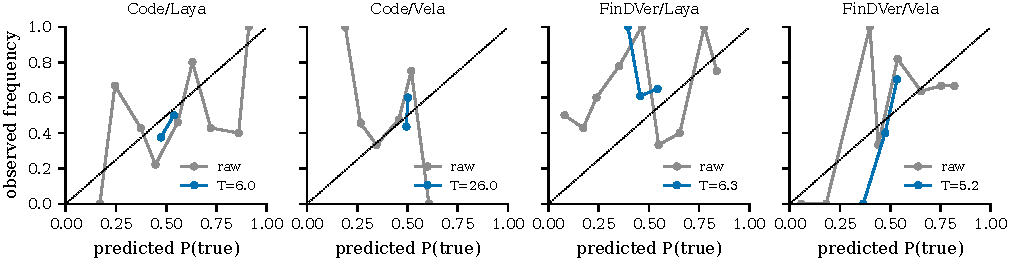
\includegraphics[width=0.96\linewidth]{../acl/figures/fig_calibration.pdf}
\caption{四个二元单元在 confirm 池上的可靠性图。灰色为原始 \noul{} 概率，
蓝色为温度缩放后。温度缩放降低校准误差，但它是单调映射：行的排序、以及
在重参数化意义下可用的带策略集合，都不变。}
\label{fig:calibration}
\end{figure}

\textbf{搜索诊断。} 图~\ref{fig:search} 汇总第~\ref{sec:results} 节讨论的
三个轨迹诊断：中性变异率、档案中训练与 dev 适应度的秩相关，以及种子 17 的
历史最优训练适应度。

\begin{figure}[t]
\centering
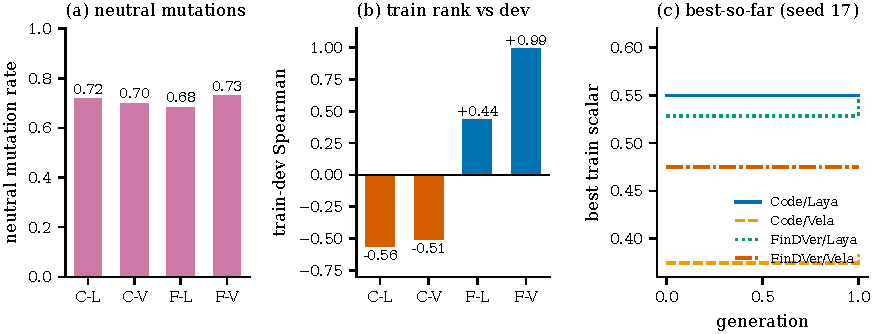
\includegraphics[width=0.96\linewidth]{../acl/figures/fig_search.pdf}
\caption{搜索诊断。(a) 68\% 到 73\% 的单基因变异不改变训练适应度。
(b) 档案中训练与 dev 适应度的秩相关在两个 CodeXGLUE 单元为负，在 FinDVer
为正。(c) 种子 17 的历史最优训练适应度；大多数运行最多改进一次，若干从
第 0 代起就平坦。}
\label{fig:search}
\end{figure}

\textbf{排序与策略价值。} 图~\ref{fig:predictability} 画出每个单元的折外
AUROC 与冻结的 dev 选择策略的 confirm 净效用。位于 0.5 右侧的点有排序信号；
位于零以下的点有负策略价值。分离清晰可见：排序信号最强的单元
（FinDVer/Vela）confirm 净值为负，而 confirm 净值最好的单元（FinDVer/Laya）
排序信号接近随机。

\begin{figure}[t]
\centering
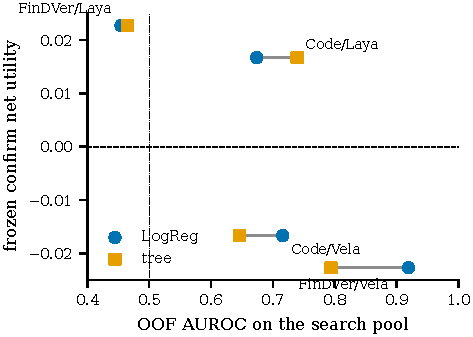
\includegraphics[width=0.78\linewidth]{../acl/figures/fig_predictability.pdf}
\caption{折外 AUROC 对 confirm 净效用。水平虚线为零净效用；垂直点线为随机
水平 AUROC。排序质量与策略价值不是同一个量。}
\label{fig:predictability}
\end{figure}

\label{app:boundary}

\textbf{边界检查。} 表~\ref{tab:boundary} 报告迁移计数与四个最高严重度的
故障图单元。图~\ref{fig:faultmap} 显示按任务、模型与置信带划分的完整
confirm 池严重度图。

\begin{table}[t]
\centering
\small
\caption{边界检查。上：冻结基因组迁移，统计相对目标固定仅切换策略的显著
配对准确率差异；对角线单元是同任务部署检查，非对角线单元是真正的迁移。
下：四个最高严重度的故障图单元，严重度定义为单元内错误率。}
\label{tab:boundary}
\begin{tabular}{@{}lrr@{}}
\toprule
迁移 & 显著正 & 显著负 \\
\midrule
对角线（同任务） & 0 & 2 \\
非对角线（真正迁移） & 0 & 4 \\
\bottomrule
\end{tabular}

\vspace{4pt}
\begin{tabular}{@{}lrrrrrr@{}}
\toprule
故障图单元 & $n$ discover & 严重度 & $n$ dev & 严重度 & $n$ confirm & 严重度 \\
\midrule
ProcessBench / Vela / 中 & 14 & 0.929 & 10 & 0.800 & 12 & 0.833 \\
ProcessBench / Laya / 中 & 13 & 0.923 & 15 & 0.867 & 16 & 0.875 \\
ProcessBench / Vela / 低 & 45 & 0.889 & 46 & 0.957 & 47 & 0.936 \\
ProcessBench / Laya / 高 & 41 & 0.756 & 35 & 0.914 & 38 & 0.895 \\
\bottomrule
\end{tabular}
\end{table}


\begin{figure}[t]
\centering
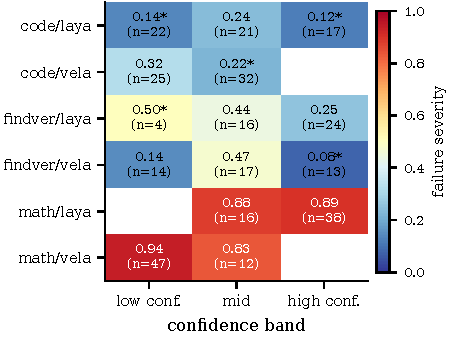
\includegraphics[width=0.78\linewidth]{../acl/figures/fig_faultmap.pdf}
\caption{按任务、模型与置信带划分的 confirm 池失败严重度。星号标记未在
0.15 容差内确认的单元。稳定的高严重度区域是 ProcessBench 的中置信度带，
两种表示在这里一起失败。}
\label{fig:faultmap}
\end{figure}

\textbf{复现细节。} 本文所有结果都来自已提交的 JSON 文件。逐行缓存是每个池
一个 JSON 文件，命名为 \texttt{cache\_<split>\_<task>\_<model>.json}，位于
\texttt{results/v4/evolution/} 下。分析脚本包括：
\begin{itemize}\setlength{\itemsep}{0pt}\setlength{\parskip}{0pt}
\item \texttt{scripts/analyze\_action\_complementarity.py}
\item \texttt{analyze\_complementarity\_heldout.py}
\item \texttt{analyze\_utility\_predictability.py}
\item \texttt{analyze\_search\_landscape.py}
\item \texttt{analyze\_transfer\_heldout.py}
\item \texttt{analyze\_calibration.py}
\item \texttt{analyze\_seed\_extension.py}
\item \texttt{analyze\_fixed\_action\_cis.py}
\item \texttt{analyze\_search\_dynamics.py}
\end{itemize}
表由 \texttt{scripts/make\_paper\_tables.py} 生成，图由
\texttt{scripts/plot\_paper\_figures.py} 生成；两个脚本都不含手抄数字。
GA/ES/NSGA-II 运行器位于 \texttt{src/evolution/}。模型修订、数据集修订、
种子与 CPU 线程数记录在每个结果文件的元数据中。五种子扩展使用种子 17、23、
41、59 与 73；预算探针使用同一缓存，唯一基因组上限为 48。不使用托管 CI
运行器：每次模型调用都在本地 Windows 机器上执行，缓存输出是本文分析的唯一
输入。

\textbf{未报告的内容。} 锁定测试未运行，\noul{} 模板未针对替代措辞审计，
没有为每个搜索策略测量真实端到端延迟，Jev 未评测。这些省略在正文中说明，
没有用代理数字填补。FinDVer/Laya confirm 单元是唯一净修复准确率区间为正的
单元；应把它视为更大规模复现的线索，而不是可部署结果。
